\documentclass[a4paper,11pt]{article}

\usepackage[utf8]{inputenc}

\usepackage{graphicx}
\usepackage{caption}
\usepackage{subcaption}

\usepackage{hyperref}

\usepackage{pgfplots}
\pgfplotsset{compat=1.18} 

\usepackage{minted}

\begin{document}

\title{
    \textbf{Assignment 12 Report - Dijkstra's Algorithm in Java}
}
\author{Dean Tsankov}
\date{\today}

\maketitle

\section*{Introduction}

In this final assignment I will present a much nicer solution to the proposed problem of the previous assignment on graphs. The conclusion we reached there was that in order to traverse a graph of nodes and find the shortest path between two specific ones, as efficiently as possible, is to keep track of all previous efforts we have done over the graph to reach a solution in optimal execution time.
This will be done here using Dijkstra's algorithm. This algorithm has the benefit of not only solving the mentioned problem, but it also records additional information regarding the shortest path to each of the nodes along the path to the one we are searching for. 
\\

This is in essence how Dijkstra's works: When we keep track of the shortest path to the nodes we have visited when we have to make a choice along which connection to go next, we will chose the one which gives the shortest distance. When this choice leads us to the destination node we will be certain that that was the shortest way to reach it. Thinking further about it this is almost the same as a breadth-first search algorithm we have implemented before, but this time in order to be able to quickly select which of the traversed nodes had the shortest path we will execute the BFS using a priority queue instead of the simple FIFO queue.

Here again in order to test the functionality we will be using a CSV file with the train lines connecting different cities. Now we are given not only the connections in Sweden, but also a larger set of cities throughout Europe so that we can gauge how much better Dijkstra's algorithm performs compared to the previous semi naive way.

\section*{Auxilary data structures}

The structures we will need here are partially similar to the ones in the previous task. The {\tt City} and the {\tt Connection} classes are almost entirely identical with the simple exception that we will now keep track of an {\tt id} value for each city, more on that later. 
\subsection*{Cities and Connections}
Generally a city now holds a name, an id and list of connections to other cities. A connection itself is the structure which holds a destination city and the value of the time to reach it.
\subsection*{Paths}
Next there is another class similar to the previous implementation - a path. The path will hold information for the distance between a current city and a destination city. One such object represents a city that is part of a path to our destination city. It therefore points to the city that is the previous step of
the complete path so there is no representation of the whole path to the destination. but instead it can be described by a sequence of path entries.
\\

Since I decide to make the {\tt Path} class a seperate file I had to also implement getter and setter functions for its properties in order to not expose them explicitly.
\begin{minted}[
frame=single,
framesep=2mm,
baselinestretch=1.2,
fontsize=\footnotesize,
]{java}
    (...)
    public class Path implements Comparable<Path>{
        private Map.City city;
        private Map.City prev;
        private Integer dist;
        private Integer index;
        public Path(Map.City currCity, Map.City prevCity, Integer dist) {
            this.index = null;
            this.city = currCity;
            this.prev = prevCity;
            this.dist = dist;
        }
        public Map.City getCity() {
            return this.city;
        }
        public Integer getIndex() {
            return this.index;
        }
        public void setIndex(Integer index) {
            this.index = index;
        }
        public void updatePath(Map.City prevCity, Integer dist) {
            this.prev = prevCity;
            this.dist = dist;
        }
        public Integer getDistance() {
            return this.dist;
        }
        @Override
        public int compareTo(Path s) {
            return Integer.compare(this.dist, s.dist);
        }
    }
    (...)
\end{minted}

\subsection*{A done array}

In order for us to be able to keep track of the progress of the algorithm there is a need to include a simple path array where we will record every node which has already been examined. This is where we will need to use the integer identifier for each city to allow us to quickly check if we had the corresponding index in the done array.  If it includes a path to city, that would mean that we had already examined that one and there would be no need to duplicate our work. Not only this, but this array will allow us to follow the shortest sequence of cities we took in order to reach our destination as each path entry has a reference to the previous city. So if we traverse them we get the complete shortest path.

\subsection*{A priority queue}
As mentioned previously for the optimal execution of this algorithm we would like to, on each iteration, select the city node which yields the shortest distance. This can ultimately be done best by utilizing a priority queue, which by its structure always keeps elements in a way where it is convenient to dequeue or poll the smallest one by some criteria, in this case - distance. We have discussed the implementation of a priority queue in class and as such I will not go into details about it here, but there was minimal modification required in order to allow it to work for our purposes in this algorithm.

\section*{The Dijkstra algorithm}

The procedure goes as follows - we want to expand our search slowly so we choose to proceed by either going to the closest immediate neighbor of our current node or to one of the neighbors of the node we came from. In the first iteration we have a single option, but on every next one this choice is left up to the priority queue which makes sure the choice is the smallest. On selecting from the queue we also need to cross reference the received path with the done array since if we had already examined the case we can ignore it. Otherwise if it has not been we add it to the done array after enqueue-ing the appropriate new path to the priority queue.
In a general sense the algorithm goes through the steps:

\begin{itemize}
    \item Poll the queue and receive a path to a city
    \item If this city is the one we are searching for, we can finish execution
    \item Otherwise if the city is not in the done array, for each of its direct connections enqueue a new path and record it as done.
\end{itemize}

In code the implementation is quite simple and should approach something like the following:

\begin{minted}[
frame=single,
framesep=2mm,
baselinestretch=1.2,
fontsize=\footnotesize,
]{java}
    (...)
    public static Result shortest(Map.City from, Map.City to) {
        PriorityQueue queue = new PriorityQueue();

        Path[] done = new Path[Map.mod];
        
        queue.enqueue(new Path(from, null, 0));

        while (!queue.isEmpty()) {
            Path fromCurrCity = queue.dequeue();
            Map.City toCity = fromCurrCity.getCity();
            Integer totalDist = fromCurrCity.getDistance();
            if (toCity.equals(to)) {
                int doneEntries = 0;
                for (Path p : done) {
                    if (p != null) {
                        doneEntries++;
                    }
                }
                return new Result(totalDist, doneEntries);
            } else {
                for (Map.Connection c : toCity.conections) {
                    if (done[c.destination.id]==null) {
                        done[c.destination.id] = new Path(c.destination,
                                toCity, c.timeToReach + totalDist);
                        queue.enqueue(done[c.destination.id]);
                    }
                }
            }
        }
        return null;
    }
    (...)
\end{minted}

The execution begins from a path to the origin city which has no previous city and a distance of zero. Next we enter a loop and perform the above described steps. Now here I am also returning the amount of entries in the done array along with the distance in a separate {\tt Result} object. This will help with benchmarking in the next section.

\section*{Gauging performance}

Let us first compare how this new algorithm fares compared to the DFS one, over the same ten city-to-city benchmarks in Sweden:


\pgfplotstableread[row sep=\\,col sep=&]{
    interval & carT & carD\\
    T1  &  92271 &   1780 \\
    T2  &  13151 &   293 \\
    T3  &  25943 &   144 \\
    T4  &  35287 &   295 \\
    T5  &  52659 &   207 \\
    T6  &  32587 &   338 \\
    T7  &  110617 &   49 \\
    T8  &  29039 &   341 \\
    T9  &  45002 &   393 \\
    T10  &  177272 &   349 \\
    }\mydata

    \begin{tikzpicture}
    \begin{axis}[
            ybar,
            bar width=.35cm,
            width=\textwidth,
            height=.5\textwidth,
            legend style={at={(0.5,1)},
                anchor=north,legend columns=-1},
            symbolic x coords={T1, T2, T3, T4, T5, T6, T7, T8, T9, T10 },
            xtick=data,
            nodes near coords = \rotatebox{90}{{\pgfmathprintnumber[]{\pgfplotspointmeta}}},
            nodes near coords align={vertical},
            ylabel={Execution in us},
        ]
        \addplot table[x=interval,y=carT]{\mydata};
        \addplot table[x=interval,y=carD]{\mydata};
        \legend{DFS, Dijkstra}
    \end{axis}
\end{tikzpicture}

There really appears to be quite the difference. But this should not surprise us when we consider how much additional unnecessary work we are cutting out of the execution by simply remembering the work we did over previous nodes in the traversal.
\\

Next we are also asked to do a benchmark where we go to measure how Dijkstra's performs on the shortest path from one specific city to a couple other random ones from the whole European data set. We do this in order to hopefully be able to somehow approximate a time complexity for the algorithm.

To be able to do this I retrieve the size of the done array for each {\tt shortest()} execution and then order the results according to it. Then that would yield the following graph showing the relation between execution time and nodes traversed.
\begin{figure}[H]
    \centering
    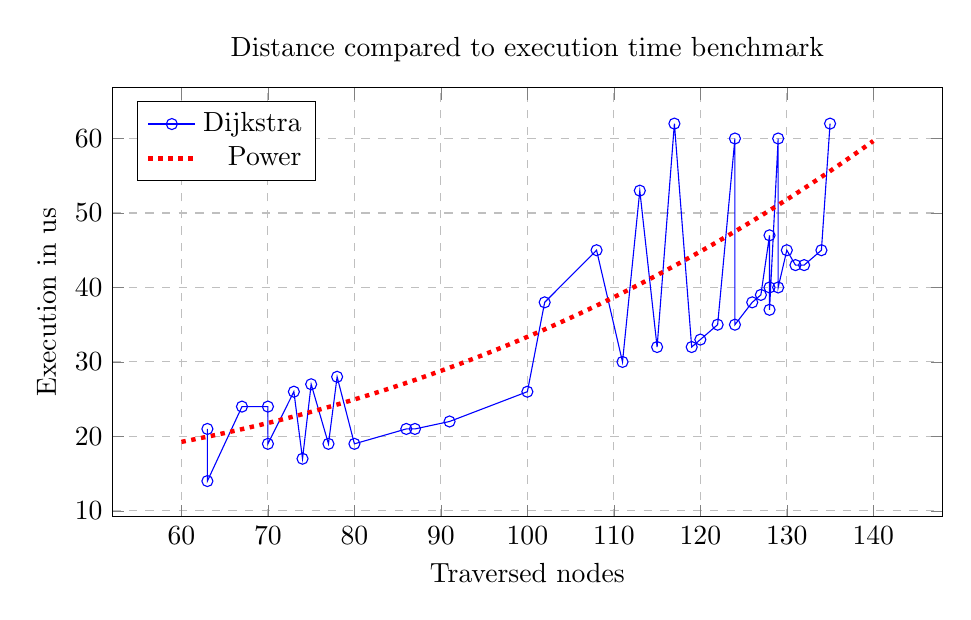
\begin{tikzpicture}
        \begin{axis}[
            title={Distance compared to execution time benchmark},
            width=\linewidth,
            height=200,
            xlabel={Traversed nodes},
            ylabel={Execution in us},
            ymajorgrids=true,
            xmajorgrids=true,
            grid style=dashed,
            legend pos=north west,
        ]
        

        \addplot[
            color=blue,
            mark=o,
            ]
            coordinates {
            (63, 21)(63, 14)(67, 24)(70, 24)(70, 19)(73, 26)(74, 17)(75, 27)(77, 19)(78, 28)(80, 19)(86, 21)(87, 21)(91, 22)(100, 26)(102, 38)(108, 45)(111, 30)(113, 53)(115, 32)(117, 62)(119, 32)(120, 33)(122, 35)(124, 60)(124, 35)(126, 38)(127, 39)(128, 47)(128, 40)(128, 37)(129, 60)(129, 40)(130, 45)(131, 43)(132, 43)(134, 45)(135, 62)
            };
            \addlegendentry[left]{Dijkstra}

        \addplot [
            domain=60:140, 
            samples=100, 
            color=red,
            dotted,
            ultra thick,
            ]
            {(x^2.55)/6500 + 14};
            
            \addlegendentry[left]{Power}
            
        \end{axis}
        \end{tikzpicture}
    \caption{Distance compared to execution time benchmark}
    \label{fig:plot1}
\end{figure}

From here we could assume a general power function appearance with relation to the number of nodes. There is definitely also some influence from the amount of edges connecting said nodes, but here since we are dealing with train lines there is a mean value of edges emerging from each node (let us say about 4) and so its influence would probably average out and not be as apparent in the performance as the number or vertices themselves.

\section*{Closing}
In conclusion, it is definitely evident that this approach to finding the shortest path over a graph, between two nodes is superior. I does not require too much additional effort to implement and the only consideration we had to make is to find out why the previous DFS algorithm performed as it did in order to negate its downfalls and improve it. Of course even in Dijkstra's there is some room for further improvement, for example if instead of using a priority queue we could use what is known as a Fibonacci heap and lower the time for operations in the queue. All in all with this we show the importance of careful consideration and methodical thinking which allows us to reach better solutions. 

The code for the implementation and ran benchmarks is uploaded in the respective \href{https://github.com/kexana/Algorithms-and-Data-Structures-ID1021}{Github repository}


\end{document}